\documentclass[wide,a4paper,titlepage,12pt] {article}
\usepackage{polski}
\usepackage[utf8]{inputenc}
\usepackage{listings}
\usepackage{slashbox}
\usepackage[table]{xcolor}
\usepackage{graphicx,pdflscape}
\usepackage{placeins}


\title{Układy cyfrowe i systemy wbudowane}
\author{Tymon Tobolski (181037)\\ Jacek Wieczorek (181043)}

% Title page layout (fold)
\makeatletter
\renewcommand{\maketitle}{
\begin{titlepage}
  \begin{center}
    \vspace*{3cm}
    \LARGE \@title \par
    \vspace{2cm}
    \textit{\small Autor:}\par
    \normalsize \@author\par \normalsize
    \vspace{3cm}
    \textit{\small Prowadzący:}\par
    Dr inż. Jarosław Sugier \par
    \vspace{2cm}
    Wydział Elektroniki\\ III rok\\ Pn 14.15 - 16.00\par
    \vspace{4cm}
    \small \@date
  \end{center}
\end{titlepage}
}
\makeatother
% Title page layout (end)



\begin{document}
\maketitle
  \section{Cel laboratorium}
  TODO
  Celem...
  \section{Zadanie nr 1}
  TODO
  Zamodelowanie .... \newline
      \begin{figure}[htbp]
	 \begin{center}
         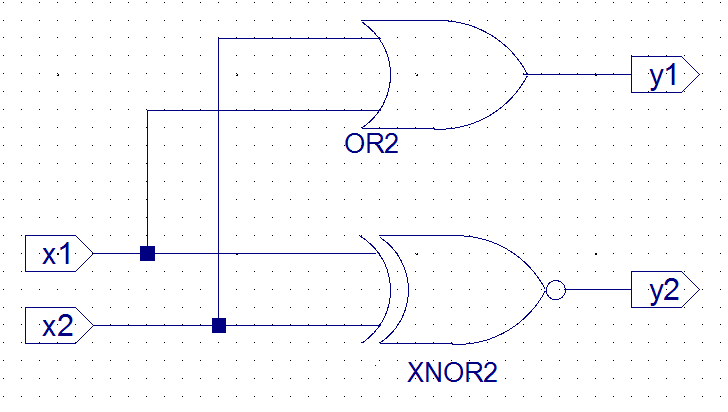
\includegraphics[scale=0.7]{pic1.PNG}
      \caption{Schemta układu}
      \end{center}
  \end{figure}
  TODO
  Następnym etapem ...
	\newpage
	\paragraph{}
	TODO
	Fragment zmodyfikowanego pliku \textit{ZL-9572.ucf} :
	\lstinputlisting[language=Vhdl]{code1.txt}

	\paragraph{}
	TODO
	Testy napisane w języku \textit{VHDL}
	\lstinputlisting[language=Vhdl]{code2.txt}


  \paragraph{}
  TODO
  Kolejnym etapem zadania było zamodelowanie działania schematu za pomocą programu ModelSim oraz zaprogramowanie urządzenia za pomocą złącza \textit{JTAG}.

  \section{Zadanie nr 2}
  TODO
  Celem ćwiczenia drugiego było zaprojektowanie, zooptymalizowanie, modelowanie i wgranie do urządzenia układu obliczającego wynik równania \textit{Y = (17-X) mod 16}. Dane wprowadzane i wyprowadzane były za pomocą magistarli cztero-wejściowej/wyjściowej. Dodatkowym zadaniem jakiego się podjeliśmy było wyświetlenie wyniku zadania na wyświetlaczu segmentowym. W celu stworzenia i zooptymalizowania układu posłużylismy się metodą siatek Karnaugh. \\
  \paragraph{}

	  \begin{center}

	  \begin{tabular}{|c|c|c||c|c|c|}
			\hline
			$Q_{2}$ & $Q_{1}$ & $Q_{0}$ & $Q_{2}'$ & $Q_{1}'$ & $Q_{0}'$ \\
			\hline
      0 & 0 & 0 & 0 & 0 & 1 \\
      0 & 0 & 1 & 0 & 1 & 1 \\
      0 & 1 & 0 & 0 & 0 & 0 \\
      0 & 1 & 1 & 1 & 0 & 0 \\
      1 & 0 & 0 & 1 & 0 & 1 \\
      1 & 0 & 1 & 1 & 1 & 0 \\
      1 & 1 & 0 & 1 & 1 & 1 \\
      1 & 1 & 1 & 0 & 1 & 0 \\
      \hline
	  \end{tabular}
	 \\ Tabela prawdy
	  \end{center}

    \begin{center}
      \begin{tabular}{|c|c|c|c|c|}
        \hline
        \backslashbox{$Q_{0}$}{$Q_{2}$$Q_{1}$} & 00 & 01 & 11 & 10 \\ \hline
        0 & 0 & 0 & \cellcolor[gray]{0.8} 1 & \cellcolor[gray]{0.8} 1 \\ \hline
        1 & 0 & \cellcolor[gray]{0.8} 1 & 0 & \cellcolor[gray]{0.8} 1 \\ \hline
      \end{tabular}
      \\ $Q_{2}'$ = $Q_{2} \bar{Q_{0}} + Q_{2} \bar{Q_{1}} Q_{0} + \bar{Q_{2}} Q_{1} Q_{0}$
    \end{center}

    \begin{center}
      \begin{tabular}{|c|c|c|c|c|}
        \hline
        \backslashbox{$Q_{0}$}{$Q_{2}$$Q_{1}$} & 00 & 01 & 11 & 10 \\ \hline
        0 & 0 & 0 & \cellcolor[gray]{0.8} 1 & 0 \\ \hline
        1 & \cellcolor[gray]{0.8} 1 & 0 & \cellcolor[gray]{0.8} 1 & \cellcolor[gray]{0.8} 1 \\ \hline
      \end{tabular}
      \\ $Q_{1}'$ = $Q_{2} Q_{1} + \bar{Q_{1}} Q_{0}$
    \end{center}

    \begin{center}
      \begin{tabular}{|c|c|c|c|c|}
        \hline
        \backslashbox{$Q_{0}$}{$Q_{2}$$Q_{1}$} & 00 & 01 & 11 & 10 \\ \hline
        0 & 0 & 0 & \cellcolor[gray]{0.8} 1 & 0 \\ \hline
        1 & \cellcolor[gray]{0.8} 1 & 0 & \cellcolor[gray]{0.8} 1 & \cellcolor[gray]{0.8} 1 \\ \hline
      \end{tabular}
      \\ $Q_{0}'$ = $Q_{2} \bar{Q_{0}} + \bar{Q_{2}} \bar{Q_{1}}$
    \end{center}



	\paragraph{}

TODO
	\begin{figure}[htbp]
	 		\begin{center}
         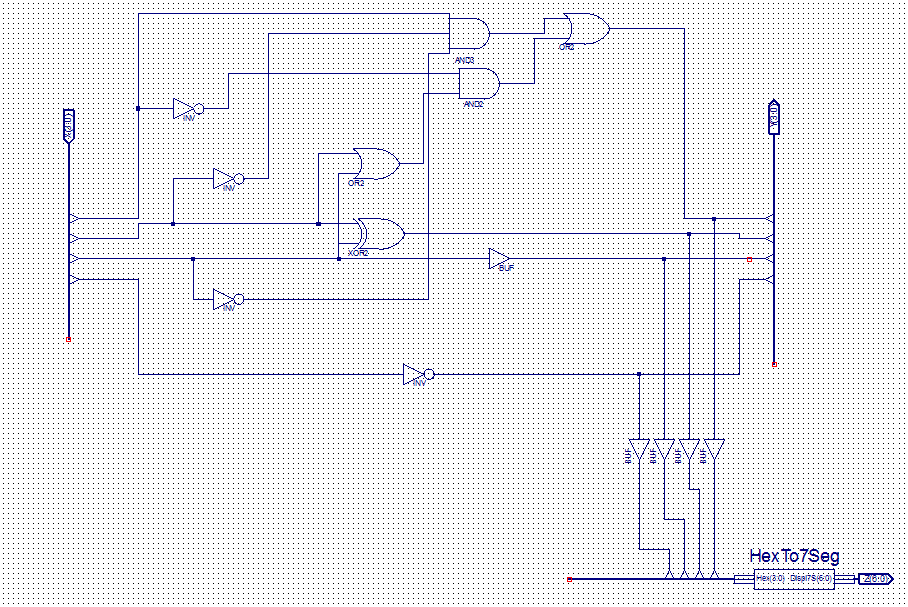
\includegraphics[scale=0.7]{pic2.PNG}
      \caption{Schemta układu}
     \end{center}
  \end{figure}

  \paragraph{}
  TODO
  Następnym etapem ćwiczenia było napisanie testów, oraz odpowiednie zmodyfikowanie pliku \textit{ZL-9572.ucf} pozwalające na zasymulowanie układu i wyświetlenie wyników na diodach oraz wyświetlaczu 7-Seg. W tym celu dołączyliśmy odpowiednią bibliotekę, pobraną ze strony kursu.
	\\ \\ \\
	\paragraph{}
	TODO
	Fragment zmodyfikowanego pliku \textit{ZL-9572.ucf} :
	\lstinputlisting[language=Vhdl]{code3.txt}

	\paragraph{}
	TODO
	Testy napisane w języku \textit{VHDL}
	\lstinputlisting[language=Vhdl]{code4.txt}

	\paragraph{}
	TODO
	Podobnie jak w przypadku pierwszego zadania, układ został najpierw zasymulowany i sprawdzony za pomocą programu ModelSim, a następnie wgrany do urządzenia i przetestowany na układzie scalonym.


  \paragraph{}
  \newpage
  \section{Wnioski}
  TODO
  Laboratorium pozwoliło nam zapoznać się z obsługą środowiska Xilinx, narzędzia do symulacji ModelSim oraz programu Impact, wgrywającego układ na płytę $ZL-9572$ za pomocą złącza $JTAG$. Dzięki edytorowi ECS, byliśmy wstanie zaprojektować układy bez znajomości języka VHDL. Ukłądy w obu zadaniach działały zgodnie z założeniami. Ze względu na specifikę elektroniczną płyty $ZL-9572$ diody zapalały się pod wpływem sygnału $\mbox{'}0\mbox{'}$, a nie jakby można by się było spodziewać $\mbox{'}1\mbox{'}$. W celu otrzymania ,,naturalnej'' reprezentacji wyjścia ($\mbox{'}1\mbox{'}$ dioda zapalona, $\mbox{'}0\mbox{'}$ - zgaszona), należałoby zanegować wszytskie bity wyjśćia.

\end{document}